\documentclass[12pt]{iopart}
%\newcommand{\gguide}{{\it Preparing graphics for IOP journals}}
\usepackage{listings}
\usepackage{minted}
\usepackage{subfig}
\usepackage{hyperref}
\usepackage{graphicx}
\usepackage{subcaption}
\usepackage[utf8]{inputenc}
\usepackage{tikz}
\usepackage[labelfont=bf]{caption}

\newminted{cpp}{gobble=2, numbersep=3pt, escapeinside=||, xleftmargin=5mm, framesep=2mm, frame=leftline, baselinestretch=1, fontsize=\scriptsize, linenos=true}
\newmintinline{cpp}{}

\makeatletter
\AtBeginEnvironment{minted}{\dontdofcolorbox}
\def\dontdofcolorbox{\renewcommand\fcolorbox[4][]{##4}}
\makeatother

\usetikzlibrary{shadows, arrows, fit, positioning, matrix, shapes}
\usetikzlibrary{decorations.markings}

% Define colors
\definecolor{my_yellow}{RGB}{255, 253, 217}
\definecolor{my_orange}{RGB}{255, 127, 0}
\definecolor{my_lightblue}{RGB}{105, 186, 249}
\definecolor{my_purple}{RGB}{150, 154, 219}
\definecolor{my_green}{RGB}{90, 194, 160}

% Define block styles  
\tikzset {
  bigbox/.style = {draw, thick, fill=gray!10, rounded corners, rectangle},
  box/.style = {draw, thick, minimum height=0.8cm, minimum width=1.5cm, rounded corners, rectangle, fill=white, anchor=south},
  model/.style = {draw, thick, fill=white, text centered, minimum height=3em, minimum width=4em, rounded corners, drop shadow},
  user/.style = {draw, thick, ellipse, fill=white, text centered, minimum height=3em, minimum width=5em, drop shadow},
  line/.style = {->, thick, color=black, shorten <=2pt, shorten >=2pt, >=stealth'},
  plain/.style = {minimum width=1em},
  %\draw [line, ->] (m1.north) ++(-15pt,-1pt) arc [start angle=-140, end angle=-400, radius=20pt] node[midway] {$T_{M_1}$} ;
  % This works around an issue with node[midway] http://tex.stackexchange.com/questions/38763/how-to-place-a-node-in-the-middle-of-an-arc                
  arcnode/.style 2 args={
    decoration={
                 raise=#1,             
                 markings,   
                 mark=at position 0.5 with {\node[inner sep=0] {#2};}
            },
            postaction={decorate}
    }
}

% Define the layers to draw the diagram
\pgfdeclarelayer{background}
\pgfdeclarelayer{foreground}
\pgfsetlayers{background,main,foreground}

% Draw background
\newcommand{\background}[5]{%
  \begin{pgfonlayer}{background}
    % Left-top corner of the background rectangle
    \path (#1.west |- #2.north)+(-0.5,0.25) node (a1) {};
    % Right-bottom corner of the background rectanle
    \path (#3.east |- #4.south)+(+0.5,-0.25) node (a2) {};
    % Draw the background
    \path[rounded corners, draw=black!50, dashed, name=box]
      (a1) rectangle (a2);
    \path (a1 |- a2) -- (a2) node[midway,below] {\large\textit{#5}};
  \end{pgfonlayer}}

% Define a circled symbol command used throughout the thesis.
\newcommand*\circled[1]{\tikz[baseline=(char.base)]{
            \node[shape=circle,draw,inner sep=2pt] (char) {#1};}}


\begin{document}

\title{Migrating large codebases to C++ Modules}

\author{Yuka Takahashi [1], Oksana Shadura [2], Vassil Vassilev [3]}
\address{[1] University of Tokyo, [2] University of Nebraska-Lincoln, [3] Princeton University}
\ead{[1] yukatkh@is.s.u-tokyo.ac.jp, [2] oksana.shadura@cern.ch, [3] vvassilev@cern.ch}

\begin{abstract}
ROOT has several features which interact with libraries and require implicit header inclusion. This can be triggered by reading or writing data on disk, or user actions at the prompt. Often, the headers are immutable and reparsing is redundant. C++ Modules are designed to minimize the reparsing of the same header content by providing an efficient on-disk representation of C++ Code. ROOT has released a C++ Modules-aware technology preview which intends to become the default for the next release.

In this paper, we will summarize our experience with migrating C++ Modules to LHC experiment's software code bases. We outline the challenges in C++ Modules migration of the CMS software, including integration of C++ Modules support in CMS build system. We also evaluate the performance benefits that experiments are expected to achieve.
\end{abstract}

\section{Introduction}
\label{intro}

In High Energy Physics (HEP), experiments such as LHC \cite{lhc} produces a large amount of data each seconds, and we expect to have even more data in Hi-lumi LHC \cite{hilumi} era. Thus software for HEP are always striving to archive the better performance, which will result in the reduction of costs in data centers as well as easing physicists waiting for their job to be processed.

ROOT~\cite{root} is a core software used in High Energy Physics (HEP) not only for data analysis, but also as a backend for larger LHC experiment's software such as CMSSW and ATLAS. Thus the performance improvement in ROOT will result in also improving experiment's software, which requires more resources than ROOT itself.

C++ Modules \cite{vassil-paper} has been supported in ROOT since version 6.16, in order to improve its performance. The cost of header re-parsing can be negligible in small to medium size codebases and very high in large codebases. Usually, the scalability issues arise at compile-time and do not affect the programs at runtime. However, ROOT is different -- its C++ interpreter Cling processes code at program execution time and avoidance of redundant content re-parsing yields better runtime performance.

The paper is divided as follows: Introduction; ...

\section{Background}

\subsection{C++ Modules in ROOT's Dictionaries}
\label{intro}

% TODO: refer this diagram

\begin{figure}[!h]
  \centering
  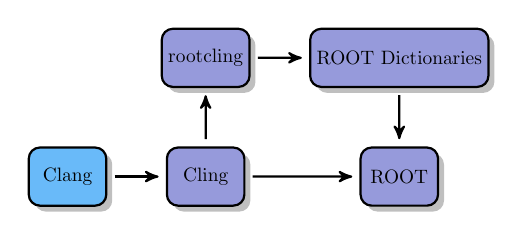
\begin{tikzpicture}[outer sep=0.05cm, node distance=0.8cm, scale=0.7, transform shape]
        
    \node[model, fill=my_lightblue, name=clang] (clang) {Clang};
    \node[model, fill=my_purple, name=cling, right=1cm of clang] (cling) {Cling};
    \node[model, fill=my_purple, name=rootcling, above=1cm of cling] (rootcling) {rootcling};
    \node[model, fill=my_purple, name=dicts, right=1cm of rootcling] (dicts) {ROOT Dictionaries};
    \node[model, fill=my_purple, name=root, below=1cm of dicts] (root) {ROOT};

    \draw[line, ->] (clang.east) -- (cling);
    \draw[line, ->] (cling.north) -- (rootcling);
    \draw[line, ->] (rootcling.east) -- (dicts);
    \draw[line, ->] (dicts.south) -- (root);
    \draw[line, ->] (cling.east) -- (root);
    
  \end{tikzpicture}
  \caption{Dependency Graph of C++ Modules in ROOT}
  \label{fig:pchandpcm}
\end{figure}

C++ Modules represent the compiler internal state serialized on disk and deserialized on demand to avoid repetitions of parsing operations, as we have described in \cite{chep-modules}. There are different implementations of the concept in Clang, GCC and MSVC. ROOT uses Clang through its interpreter Cling and adopts the C++ Modules implementation in Clang[FIXME:CITE CLANG MODULES], which is one of the most sophisticated on the market as of today.

Many operations in ROOT require loading a shared library and its corresponding header files. For example when we serialize or deserialize a ROOT file, ROOT needs to know which library contains how to stream the object. This meta information is widely known as ROOT "dictionary" information. The dictionary is generated by a platform-independent tool, \textit{rootcling}, which processes ROOT-aware code and produces C++ source code file with a prefix \textit{G\_\_}. The file is later compiled and linked into the library it describes.

Generally, there are two ways to load a library: implicitly or explicitly. Both models require the library description to be available before or no later than library loading time. That is, all header files describing the library should be processed by the interpreter blindly without knowing if they will be used. This is a severe performance bottleneck which ROOT addresses with several technologies: \textit{ROOTMAP}s, \textit{RDICT}s and a \textit{PCH}. The ROOTMAP file represents a lightweight version of the library descriptor containing forward declarations and their mapping to the corresponding library. The RDICT file represents a cache of a subset of \textit{TClass} objects which will be created when the library is loaded. The PCH file contains almost all of the headers in ROOT in an optimized form which is loaded at start up to avoid header re-parsing.

The ROOTMAPs and RDICTs are home-grown fixes to the inherent PCH problem -- it is impossible to extend a PCH without fully recompiling it. C++ Modules are the industry solution to this problem -- they represent composable PCH files called \textit{PCM}s.

A PCM is generated by rootcling using a special file containing the mapping between a header file and the module to be created, called a \textit{modulemap} file. It describes how a collection of existing headers corresponds to the logical structure of a module. It is important to note that transitive includes not present in a modulemap file are persisted multiple times. That is, if \textit{A.h} includes \textit{C.h}, \textit{B.h} includes \textit{C.h} and the modulemap maps A.h to module \textit{Alpha} and B.h to module \textit{Beta}, the content of C.h will be duplicated in both Modules. Such duplication can reduce performance dramatically and should be avoided at almost any cost. This important detail suggest that "modularization" should be done bottom-up, namely, starting from external dependencies onward.

%Third-party code can work in mixed mode with ROOT with enabled C++ Modules. For instance, the dictionaries of CMSSW can use the old dictionary system while the dictionaries of ROOT use the new technology. Ultimately, this will not manifest into performance improvements because the C++ Modules technology intends to address dictionaries outside of the ROOT PCH, namely, in third-party software. The mixed mode support ensures an incremental migration path while having a stable system throughout the migration period. 

\subsection{Overview of CMSSW}
\label{cmssw}

\begin{figure}[!h]
  \centering
  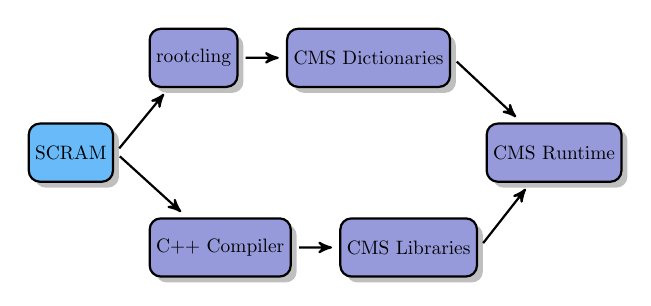
\begin{tikzpicture}[outer sep=0.05cm, node distance=0.8cm, scale=0.7, transform shape]
        
    \node[model, fill=my_lightblue, name=scram] (scram) {SCRAM};
    \node[model, fill=my_purple, name=compiler, below right=of scram] (compiler) {C++ Compiler};
    \node[model, fill=my_purple, name=rootcling, above right=of scram] (rootcling) {rootcling};
    \node[model, fill=my_purple, name=dicts, right=of rootcling] (dicts) {CMS Dictionaries};
    \node[model, fill=my_purple, name=libs, right=of compiler] (libs) {CMS Libraries};
    \node[model, fill=my_purple, name=cms, above right=of libs, below right=of dicts] (cms) {CMS Runtime};

    \draw[line, ->] (scram.east) -- (rootcling);
    \draw[line, ->] (scram.east) -- (compiler);
    \draw[line, ->] (compiler.east) -- (libs);
    \draw[line, ->] (rootcling.east) -- (dicts);
    \draw[line, ->] (dicts.east) -- (cms);
    \draw[line, ->] (libs.east) -- (cms);
    
  \end{tikzpicture}
  \caption{Dependency Graph of C++ Modules in CMSSW}
  \label{fig:pchandpcm}
\end{figure}

CMS \cite{cms} is one of the largest experiment in LHC and performance improvement of its software is crucial for the coming HL-LHC. CMS experiment develops their software stack called CMSSW (CMS SoftWare)[FIXME: CITE CMSSW WEBSITE or PAPER] which uses ROOT as its backend.

CMSSW utilizes their own build system, SCRAM \cite{scram}. SCRAM is a configuration management tool, a distribution system, a build system and a resource manager, with local resources and applications managed in a transparent way. Enabling C++ Modules in SCRAM is a crucial part of the project.

% TODO: reference the CMSSW diagram
In CMSSW, SCRAM build system resolves library dependencies and executes and also C++ compiler such as gcc ROOT Genreflex, which is a wrapper of rootcling. Rootcling generates CMS ROOT dictionaries, rootmaps and RDICTs, as it was in ROOT. At the same time gcc compiles C++ files and generates CMS shared object libraries. 

\section{Migrating CMSSW to C++ Modules}
\label{migration}

%FIXME: In CMSSW, SCRAM generates modulemap for only libraries which has --cxxmodule flag enabled. it iterates through interface/ directory, add header files in them and automatically generates classes.h. Generate modulemap, pcms, and load them.
Modularizing CMSSW requires two steps: generating a modulemap file and enabling C++ Modules in \textit{rootcling}. The generation of modulemap file happens at configuration time where we produce a file describing each library as a module and each library header file as a submodule. This can be subtle in some build systems as it requires tracking of header files which usually is not required. SCRAM already supports this and it was trivial to synthesize that description. Enabling C++ Modules in rootcling is done by adding an extra \textit{-cxxmodule} flag. We started doing that gradually library-by-library to avoid unnecessary complications.

This section describes the steps taken in CMSSW in order to migrate fully to C++ Modules. We mention a few items of work which are complete, a few which are ongoing and in both cases the work was conducted by the authors but with significant support of our colleagues mentioned in section \ref{ack}.

\subsection{Autogeneration of modulemap}
% This section is probably the most important section in this paper, as all other experiments' librarian wants to know how they can modularize their software stack.

% describe how scram generates modulemap here in deail. Also we can mention about classes.h
As was mentioned in the section \ref{intro}, one of important features to be adjusted is generation modulemaps. As you can imagine, modulemap could contain all interface header files in the end, and can be quite large and become hard to maintain by hand. This is why we need to autogenerate the module map, which will be explained in next slides.

Autogeneration of module map is quite simple. CMSSW has interface headers, which is exposed to outside libraries. We automatically generate the modulemap by iterating through those interface headers. Modulemap needs to be generated before any execution of genreflex, so it needs to happen at configuration time of CMSSW.
We rely on SCRAM for generation modulemap. This module map is used by Genreflex to generate CMS PCMs, and also at CMS runtime.

% FIXME: SCRAM already has a dependency list according to which it determines the order of genreflex execution. If a header was included in other modules without explicit dependency, it's a problem.
\subsection{Header Sanitizing}
In most cases, a module corresponds to a single dictionary (or library). Each module enumerates every header file in a submodule. Each submodule needs to be able to compile in isolation. Illustratively, a separate compiler instance is run on each header file. This assumes that every header file should be able to compile on its own. \textit{Standalone} header files include what they use and are resilient to configuration macros.

CMSSW codebase had a lot of header files inaccuracies thoroughly described in the GitHub C++ Modules Meta Issue~\cite{Modules-gh-metaissue}. The issues can be classified into the following categories:
\begin{itemize}
    \item Incomplete headers -- header files which do not include what they use. They are easy to fix because the C++ Modules system usually is able to suggest which are the omitted includes;
    \item Broken headers -- header files which never compiled. Those header files were never included in any translation unit but were "part" of a library. They are easy to deprecate and remove;
    \item Cyclic headers -- header files whose include graph contains a cycle. For example, header \textit{A} includes header \textit{B} which includes \textit{A}. Header \textit{A} is in module \textit{Alpha} and header \textit{B} in \textit{Beta}. Usually this is a signal for a layering violation -- concepts from one library depend on another an vice versa. In many cases, using forward declarations of such entities resolve the problem. In some cases more sophisticated engineering techniques are necessary, such as, refactoring, moving the two dependent headers together or splitting the common dependent logic into its own library and module. In rare cases, if the mutual dependence of headers is by design they have to be in a single submodule.
    \item Macro headers -- header files which contain predominantly macro definitions which can be expanded differently in each translation unit. For example, \textit{$<$assert.h$>$} which conditionally defines the \textit{assert} if \textit{NDEBUG} is not defined. Macro headers are meant to be always textually included and they should be marked as \textit{textual headers} in the modulemap file. 
    \item Token generating headers -- header files which enable preprocessor metaprogramming should be excluded from the modulemap file.
\end{itemize}

After sanitizing the header files a toolchain to protect regressions can be introduced. In CMSSW every header in a pull request is checked for the aforementioned issues. This is done by precompiling each header on its own. In future we will deploy the include graph sanitization tool which we used to detect include cycles~\cite{scram-cycle-break}.

\subsection{Virtual Modulemap Overlay}

\begin{figure}[!h]
  \centering
  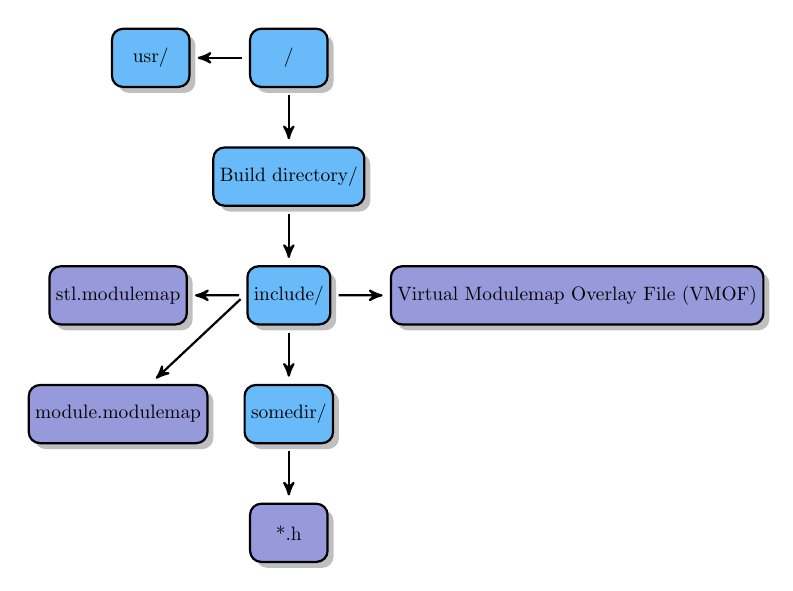
\begin{tikzpicture}[outer sep=0.05cm, node distance=0.8cm, scale=0.7, transform shape]
        
    \node[model, fill=my_lightblue, name=root] (root) {/};
    \node[model, fill=my_lightblue, name=usr, left=1cm of root] (usr) {usr/};
    \node[model, fill=my_lightblue, name=build, below=1cm of root] (build) {Build directory/};
    \node[model, fill=my_lightblue, name=inc, below=1cm of build] (inc) {include/};
    \node[model, fill=my_lightblue, name=somedir, below=1cm of inc] (somedir) {somedir/};
    \node[model, fill=my_purple, name=headers, below=1cm of somedir] (headers) {*.h};
    \node[model, fill=my_purple, name=stlmodmap, left=1cm of inc] (stlmodmap) {stl.modulemap};
    \node[model, fill=my_purple, name=modmap, below=1cm of stlmodmap] (modmap) {module.modulemap};
    \node[model, fill=my_purple, name=virtmap, right=1cm of inc] (virtmap) {Virtual Modulemap Overlay File (VMOF)};

    \draw[line, ->] (root.west) -- (usr);
    \draw[line, ->] (root.south) -- (build);
    \draw[line, ->] (build.south) -- (inc);
    \draw[line, ->] (inc.south) -- (somedir);
    \draw[line, ->] (somedir.south) -- (headers);
    \draw[line, ->] (inc.west) -- (stlmodmap);
    \draw[line, ->] (inc.west) -- (modmap);
    \draw[line, ->] (inc.east) -- (virtmap);
    
  \end{tikzpicture}
  \caption{Modulemap infrastructure for ROOT and CMSSW.}
  \label{fig:modulemap}
\end{figure}

% FIXME!: put diagram for module maps here
Let’s take a closer look to module map system. In the diagram \ref{fig:modulemap} is shown organization of C++ Modules infrastructure together with module map system. Here circles corresponds to directories and squares corresponds to files. Imagine the top circle means root directory. As said, module map file needs to be placed where the header files exist. So in this example, it needs to know where the *.h header files exist.

However, there is some problems in module map system.  For example, we want to enable C++ Modules for system headers. It means that for system headers, for example \textit{STL} and \textit{libc} module maps don’t exist by default. Thus we need to provide module map by ourselves. Module map system itself does not solve this complex situation, that’s why we need to introduce module map overlay file.

Module map overlay file is generated at the configuration time and gives Clang the important information of the location of system headers and the relative path to \textit{stl} module map. System module maps, for example the \textit{stl} module map has a similar contents as \textit{module.modulemap}. From modulemap overlay file and \textit{stl.modulemap}, Clang combines those information and treat internally as it is modulemap existing in \textit{usr/include}. However, it also has the downside that it needs to be generated at the configuration time.

% FIXME!!: Why there is no virtual modulemap overlay?

\subsection{Modularizing External Dependencies}

In order to fully see the expected performance benefits we should modularize external dependencies as well. An external dependency should be modularized if a module transitively includes it. For example if header \textit{A} from module \textit{Alpha} includes directly or indirectly \textit{$<$vector$>$}, the external library, \textit{libstdc++}, containing that file should be modularized.

It can be challenging to modularize external dependencies. On the one hand it may be difficult to know what the modulemap file should contain. On the other hand because they can be in a non-writable locations on the file system. We have prepared a set of modulemap files for all external dependencies of CMSSW~\cite{raphael-auto-Modules}. The second challenge is solved a file which instructs rootcling to pretend that the modulemap file is located at the non-writable folder in the file system. The \textit{virtual file system overlay file} can be automatically synthesized by~\cite{raphael-auto-Modules}.


\section{Preliminary Results}
\label{results}
FIXME: Explain we are still running in mixed mode.
In \ref{fig:perf:a},\ref{fig:perf:b},\ref{fig:perf:c} and \ref{fig:perf:d} are shown results of benchmarks from CMSSW testing suite with enabled C++ Modules. On \ref{fig:perf:a} is shown a benchmark of ESetup Lock in Fast simulation test. ESetup is auxiliary information needed to process an Event. The left bar is ROOT Master, with no Modules. The middle bar is a ROOT with only ROOT PCMs, which means that we're not loading PCMs from CMSSW in this build. The right bar is ROOT PCMs + CMS PCMs, which is loading 121 PCMs in total. As you can see, CMS PCMs build runs 22.5 seconds better than ROOT Master.

\ref{fig:perf:b} is shown results of benchmark of ESetup Get in Fast simulation test. In this test, CMS PCMs build was 15.2 seconds fater than ROOT Master.
\ref{fig:perf:c} is shown results of benchmark of CPU Total Loop in Digitization test. CMS PCMs build was 331 seconds faster than ROOT Master.
\ref{fig:perf:d} is shown results of benchmark of RSS in Digitization test. CMS PCMs build had 143 MBytes worse RSS than ROOT Master.

\begin{figure}
\centering
\begin{minipage}{.48\textwidth}
\subfloat[] {\label{fig:perf:a} \includegraphics[width=\textwidth]{0.png}}
\end{minipage}\hfill
\begin{minipage}{.48\textwidth}
\subfloat[] {\label{fig:perf:b} \includegraphics[width=\textwidth]{1.png}}
\end{minipage}
\begin{minipage}{.48\textwidth}
\subfloat[] {\label{fig:perf:c} \includegraphics[width=\textwidth]{2.png}}
\end{minipage}\hfill
\begin{minipage}{.48\textwidth}
\subfloat[] {\label{fig:perf:d} \includegraphics[width=\textwidth]{3.png}}
 \end{minipage}
 \caption{Performance results: (a) is the ESetup Lock RT time measurements. (b) is showing the ESetup RT  measurements. (c) is showing the 250199.18 CPU total loop measurements. (d) is showing the 500199.0 RSS measurements.}
\label{fig:performance1}
\end{figure}
 
 The work presented in this article shows that C++ Modules technology were successfully implemented and tested in ROOT and CMSSW software framework. The work on performance improvement is still ongoing. C++ Modules will provide experiments a benefit of header modularity of libraries and performance improvement.

\section{Limitations and Future work}
% TODO: Not all CMS libraries were modularized?:
\begin{enumerate}
    \item Incremental builds -- building ROOT, modifying the source code and rebuilding might not work. To work around it remove all PCM files in the build folder.
    \item Relocatability issues -- we have fixed a few of the relocatability issues we found. We are aware of an obscure relocatability issue when ROOT is copied in another folder and we are rebuild. ROOT picks up both modulemap files in seemingly distinct locations.
    \item Building PCMs with rootcling -- in rare cases there might be issues when building PCM files with rootcling. The easiest will be to open a bug report to clang, however, reproducing a failure outside of rootcling is very difficult at the moment.
    \item Generation of some dictionary hangs -- on some platforms (depending on the version of libstdc++) the generation of the dictionary goes in an infinite loop. 
    \item Layering violations in some ROOT components.
\end{enumerate}


\section{Acknowledgments}
\label{ack}

This work has been supported by an Intel Parallel Computing Center grant, by U.S. National Science Foundation grants PHY-1450377, ACI-1450323 and PHY-1624356, and by the U.S. Department of Energy, Office of Science.

The authors are thankful to Shahzad Malik Muzaffar and Mircho Rodozov from the CMSSW devops team.

The authors would like to thank CERN/EP-SFT and the ROOT team in particular.


\section*{References}

\begin{thebibliography}{10}

\bibitem{lhc}
Lyndon Evans and Philip Bryant, LHC Machine, Journal of Instrumentation,IOP Publishing,Volume 3, 08, S08001--S08001, DOI:10.1088/1748-0221/3/08/s08001

\bibitem{hilumi}
The HL-LHC Project. 2019. The HL-LHC Project | High Luminosity Large Hadron Collider. [ONLINE] Available at: http://hilumilhc.web.cern.ch/. [Accessed 15 May 2019]. 

\bibitem{root}
R. Brun, F. Rademakers, ROOT - An Object Oriented Data Analysis Framework, Nucl. Inst. \& Meth. in Phys. Res. A, 389, (Proceedings AIHENP'96 Workshop,1997).

\bibitem{vassil-paper}
Vassil Vassilev, Optimizing ROOT's Performance Using C++ Modules, Journal of Physics: Conf. Ser., 898, 072023 (2017)

\bibitem{chep-modules}
Yuka Takahashi and al., Optimizing Frameworks Performance Using C++ Modules Aware ROOT, CoRR, arXiv:1812.03992 [cs.PL]

\bibitem{cms}
CMS Collaboration,CMS: The computing project. Technical design report, CERN-LHCC-2005-023.

\bibitem{scram}
GitHub. 2019. GitHub - cms-sw/SCRAM: Software Configuration And Management - CMS internal build tool. [ONLINE] Available at: https://github.com/cms-sw/SCRAM. [Accessed 15 May 2019]. 

\bibitem{Modules-gh-metaissue}
GitHub. 2019. C++ Modules support (based on Clang) - Issue 15248 -cms-sw/cmssw GitHub. [ONLINE] Available at: https://github.com/cms-sw/cmssw/issues/15248. [Accessed 15 May 2019]. 

\bibitem{scram-cycle-break}
GitHub. 2019. Circle Break - Teemperor/circle-break. [ONLINE] Available at: https://github.com/Teemperor/circle-break. [Accessed 15 May 2019]. 

\bibitem{raphael-auto-Modules}
GitHub. 2019. GitHub - Teemperor/ClangAutoModules: Automatically mounts clang modules for your system libraries (and more). [ONLINE] Available at: https://github.com/Teemperor/ClangAutoModules. [Accessed 15 May 2019]. 

\end{thebibliography}

\end{document}